\chapter{Test Journal: Force-PWM Relation}\label{app:forceTest}

\textbf{Date: 10/05/2017}

\subsection*{Purpose}
The purpose of this test journal is to find the relationship between the command sent to the LLI and the force that the propellers apply.

%\subsection{Theory}
%By knowing the Force applied to the vessel and the acceleration, the added mass can be obtained by rearranging equation \autoref{eq:x_pos_model} and \autoref{eq:y_pos_model} to acquire the x and y components respectively.
%This assumes the force-input relationship of the actuators as well as the drag coefficients is known.

\subsection*{Equipment}
\begin{itemize}
	\item Vessel with all its components.
%	\item Emlid Reach RTK GPS
%	\item 2x INLINE 750 14.8V brushless DC-Motor
%	\item 2x Speed Controller +70 G3.5
%	\item ADIS16405BMLZ IMU
%	\item Ps3 Controller  
	\item External laptop.
    \item Newton meter, AAU number 02054-03.
\end{itemize}

%%%% Test Setup
\subsection*{Procedure}
\begin{enumerate}
	\item Turn on all equipment.
    \item Remotely log into the boat, when both, laptop and vessel's computer, are in the same network.
	\item Run the following nodes
		\begin{itemize}
			\item \lstinline[style=cinline]{/lli_node}
			\item \lstinline[style=cinline]{/keyboard_teleop_node}
		\end{itemize}
    \item Send a PWM command to the LLI and measure the resultant force.
	\item Move the vessel using the keyboard.
    \item Repeat previous step with other commands, both positive and negative.
    \item Process the data
\end{enumerate}


\subsection*{Results}
The relation between force and PWM command depends on the sign of the force, as can be seen in \autoref{fig:F_pos} and \ref{fig:F_neg}.
\begin{figure}[H]
    \captionbox 
    {   
        Plot of the relation between positive force and PWM command.
        \label{fig:F_pos}
    }                                                                 
    {                                                                  
        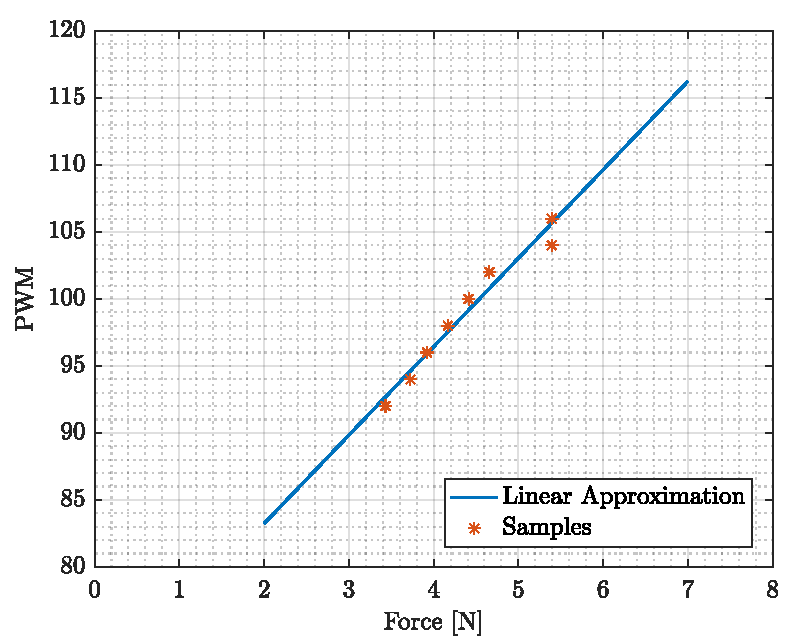
\includegraphics[width=.45\textwidth]{figures/F_pos}         
    }                                                                    
    \hspace{5pt}                                                          
    \captionbox  
    {      
        Plot of the relation between negative force and PWM command.
        \label{fig:F_neg}
    }                                                                          
    {
        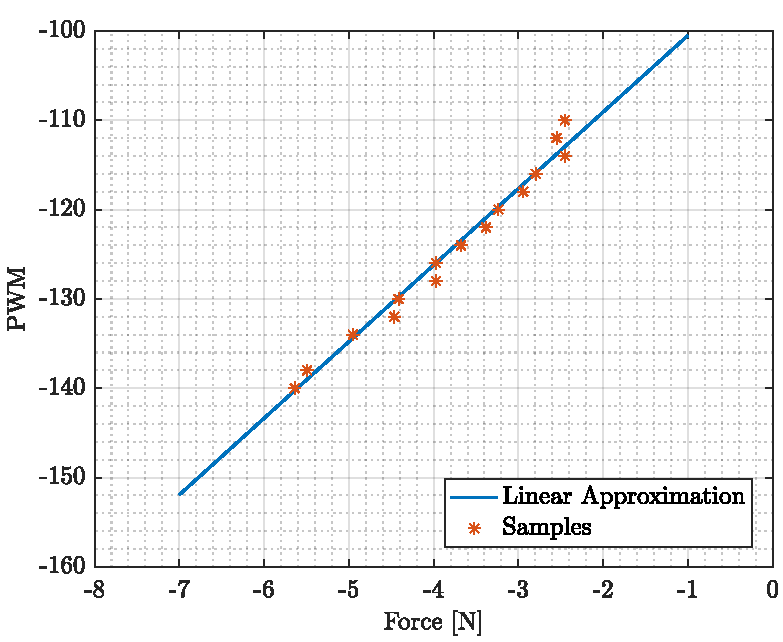
\includegraphics[width=.45\textwidth]{figures/F_neg}
    }
\end{figure}

For positive forces, the relation is as follow
\begin{flalign}
    \mathrm{PWM} = \num{6.6044} \ F + \num{70.0168} \ \ .
\end{flalign}

For negative forces, the relation is as follows
\begin{flalign}
    \mathrm{PWM} = \num{8.5706} \ F - \num{91.9358} \ \ .
\end{flalign}


